\documentclass[conference]{IEEEtran}

\usepackage{amsmath}
\usepackage{booktabs}
\usepackage{graphicx}
\usepackage{tabularx}
\usepackage{array}
\usepackage{microtype}
\usepackage{cite}
\usepackage{placeins}
\usepackage[hidelinks]{hyperref}

\hypersetup{
    pdfauthor={},
    pdftitle={Communication-Aware Federated Brain Tumor MRI Classification},
    pdfsubject={},
    pdfkeywords={},
    pdfcreator={},
    pdfproducer={}
}
\ifdefined\pdfinfoomitdate
    \pdfinfoomitdate=1
\fi
\ifdefined\pdftrailerid
    \pdftrailerid{}
\fi
\ifdefined\pdfsuppressptexinfo
    \pdfsuppressptexinfo=-1
\fi

\newcolumntype{L}[1]{>{\raggedright\arraybackslash}p{#1}}
\newcolumntype{C}[1]{>{\centering\arraybackslash}p{#1}}
\newcolumntype{Y}{>{\raggedright\arraybackslash}X}

\title{Communication-Aware Federated Brain Tumor MRI Classification}
\author{\IEEEauthorblockN{Anonymous Authors}}

\begin{document}
\maketitle

\begin{abstract}
Reliable comparison of federated brain tumor MRI backbones requires control of data leakage, partition variability, and statistical uncertainty. We present a duplicate-controlled evaluation protocol for communication-aware federated classification that combines cluster-aware splitting, matched client assignments, repeated seeds, and paired fixed-test-set analysis. Exact, pixel-level, and conservative near-duplicate images are grouped before a balanced train--validation--test split is constructed, and five ImageNet-pretrained backbones are screened by validation macro-F1. The selected EfficientNet-B0 and a ResNet50 baseline are then compared under the same Non-IID FedAvg schedule across seeds 42, 123, and 2025. EfficientNet-B0 achieved $97.25\pm0.51$\% accuracy and macro-F1, compared with $97.18\pm0.28$\% for ResNet50. Paired analyses did not detect a statistically distinguishable difference for any seed. EfficientNet-B0 reduced full-state communication payload per 20-round run from 14,385.65~MiB to 2,474.84~MiB, approximately 82.8\% lower. By controlling major experimental confounders, the protocol supports a more defensible interpretation of this accuracy--payload tradeoff; the results do not support a claim of accuracy superiority.
\end{abstract}

\begin{IEEEkeywords}
federated learning, brain tumor MRI, communication efficiency, duplicate control, medical image classification
\end{IEEEkeywords}

\section{Introduction}
Federated learning (FL) allows several clients to train a shared classifier without pooling their raw images in one location \cite{mcmahan2017fedavg,rieke2020future}. Brain tumor MRI classification is a common four-class benchmark for this setting \cite{nickparvar_brain_tumor_mri,bentemessek2025brain,khatoon2026resnet50,ghanta2025federated}. Yet a useful federated comparison must answer more than which model records the highest test accuracy. It must also show that the split is credible, that the result survives changes in random seed, and that communication is measured under the same protocol.

Split integrity is especially important for public MRI collections. Exact duplicates, transformed copies, and highly similar slices may otherwise appear on both sides of an evaluation boundary, producing optimistic test estimates \cite{melo2026exploiting,siam2026brain,naseer2026medfl}. Repeating an experiment across seeds cannot repair leakage already built into the split. Related images must be grouped before any backbone or federated method is compared.

Model size creates a separate practical tradeoff. In full-state FL, every participating client downloads and uploads the complete model state in each round \cite{mcmahan2017fedavg,radhika2026communication,zhou2022communication}. When data splitting, client partitioning, optimization, and backbone architecture vary simultaneously, communication--performance tradeoffs become difficult to attribute. This study isolates backbone choice by holding the duplicate-controlled split, client participation, optimization, round schedule, and evaluation procedure fixed. The comparison concerns tensor payload, not algorithmic compression, end-to-end network performance, or privacy guarantees.

Figure~\ref{fig:pipeline} shows the study design. We first group exact, resized-pixel, and conservative same-class near duplicates, then build one balanced cluster-aware split. Five pretrained backbones are screened centrally using validation macro-F1. Finally, EfficientNet-B0 and ResNet50 are evaluated with the same 20-round Non-IID FedAvg schedule. Within each of three seeds, the two models load the same saved client assignment, so partition variation is not confounded with backbone choice.

The resulting accuracy difference is small, whereas the calculated payload difference is large. EfficientNet-B0 achieved $97.25\pm0.51$\% mean accuracy and ResNet50 achieved $97.18\pm0.28$\%; fixed-test-set analyses found no statistically distinguishable difference for any seed. Their full-state communication payloads were 2,474.84 and 14,385.65~MiB per run, respectively. Because the client count and round schedule are fixed, this payload difference follows directly from model state size. The approximately 82.8\% reduction supports compact-backbone selection in this simulation, but it does not establish statistical equivalence or clinical readiness.

The contributions are:
\begin{itemize}
    \raggedright
    \setlength{\itemsep}{0.15em}
    \setlength{\parsep}{0pt}
    \item \textbf{Duplicate-controlled evaluation protocol:} cluster-aware grouping before splitting, yielding zero detected exact, resized-pixel, or conservative near-duplicate cross-split overlaps under the stated criteria.
    \item \textbf{Statistically rigorous federated evaluation:} matched client assignments, three repeated seeds, stable prediction alignment, exact McNemar tests, and class-stratified paired bootstrap intervals.
    \item \textbf{Communication-aware backbone comparison:} EfficientNet-B0 and ResNet50 evaluated under identical federated optimization, participation, and round schedules, with accuracy interpreted jointly with full-state payload per run.
\end{itemize}

\section{Related Work}
\subsection{Federated Learning for Medical Imaging}
FedAvg remains the standard FL baseline: clients optimize locally, and the server averages their updates in proportion to local sample counts \cite{mcmahan2017fedavg}. FedProx adds a proximal term to limit local drift when client data are heterogeneous \cite{li2020fedprox,ghanta2025federated}. Both protocols and their variants have been studied for tumor classification, glioma detection, and segmentation \cite{sharma2025privacy,mastoi2025explainable,saraswat2026hybrid,wakili2025twinsegnet}. Among the closest task-specific studies, Ghanta et al. emphasize FedProx with augmentation under heterogeneous partitions \cite{ghanta2025federated}, whereas Melo et al. study preprocessing and test-time augmentation \cite{melo2026exploiting}. Our focus is instead duplicate-controlled splitting followed by a matched, repeated backbone comparison with paired prediction-level analysis. Most public-dataset studies, including ours, simulate clients rather than observe independent hospitals. Such partitions cannot reproduce institutional differences in scanners, populations, acquisition protocols, or governance \cite{rieke2020future,xu2023federated,naseer2026medfl}. We therefore use four virtual clients to study a controlled backbone tradeoff, not institutional generalization.

\subsection{Brain Tumor MRI Classification and Dataset Reliability}
The Nickparvar collection contains glioma, meningioma, no-tumor, and pituitary MRI classes and is widely used to compare CNN backbones and FL protocols \cite{nickparvar_brain_tumor_mri,bentemessek2025brain,khatoon2026resnet50,ghanta2025federated}. ResNet50 provides a familiar high-capacity baseline \cite{he2016resnet}, whereas EfficientNet uses compound scaling to obtain a smaller model \cite{tan2019efficientnet}. On this dataset family, however, the split can matter as much as the backbone. Work on medical-image leakage motivates duplicate removal and patient-wise or cluster-aware partitioning before evaluation \cite{melo2026exploiting,siam2026brain}. Our split follows that principle by keeping detected exact, resized-pixel, and conservative same-class near-duplicate groups intact.

\subsection{Communication and Backbone Efficiency}
Communication-efficient FL often changes the transmitted update through sparsification, quantization, or restricted uploading \cite{radhika2026communication,aniket2025cfl,zhou2022communication,das2026federated}. Backbone choice acts earlier in the pipeline. If every round exchanges full states, payload grows directly with state size, client participation, and the number of rounds. EfficientNet-B0 is already used as a lightweight medical-imaging backbone \cite{tan2019efficientnet,abubakr2026explainable}; the unresolved question is whether its smaller state remains competitive under the same split and FL schedule as a heavier model. We address that question through repeated matched runs and explicit full-state payload accounting, not a new compression method.

The studies reviewed above emphasize FL algorithms, augmentation, backbone architectures, or transmitted-update reduction. Our distinction is to combine detected-duplicate control, matched per-seed client assignments, repeated runs, paired prediction-level statistics, and per-run payload accounting within one evaluation protocol. This joint control makes the observed accuracy--payload tradeoff attributable to backbone choice within the tested setting.

\section{Methodology}
The study has four steps, shown in Fig.~\ref{fig:pipeline}: construct one duplicate-controlled split, screen candidate backbones on validation data, run federated experiments with saved client assignments, and account for every uploaded and downloaded model state. Keeping these steps separate prevents test data, partition variation, and model size from becoming hidden confounders.

\begin{figure*}[!t]
\centering
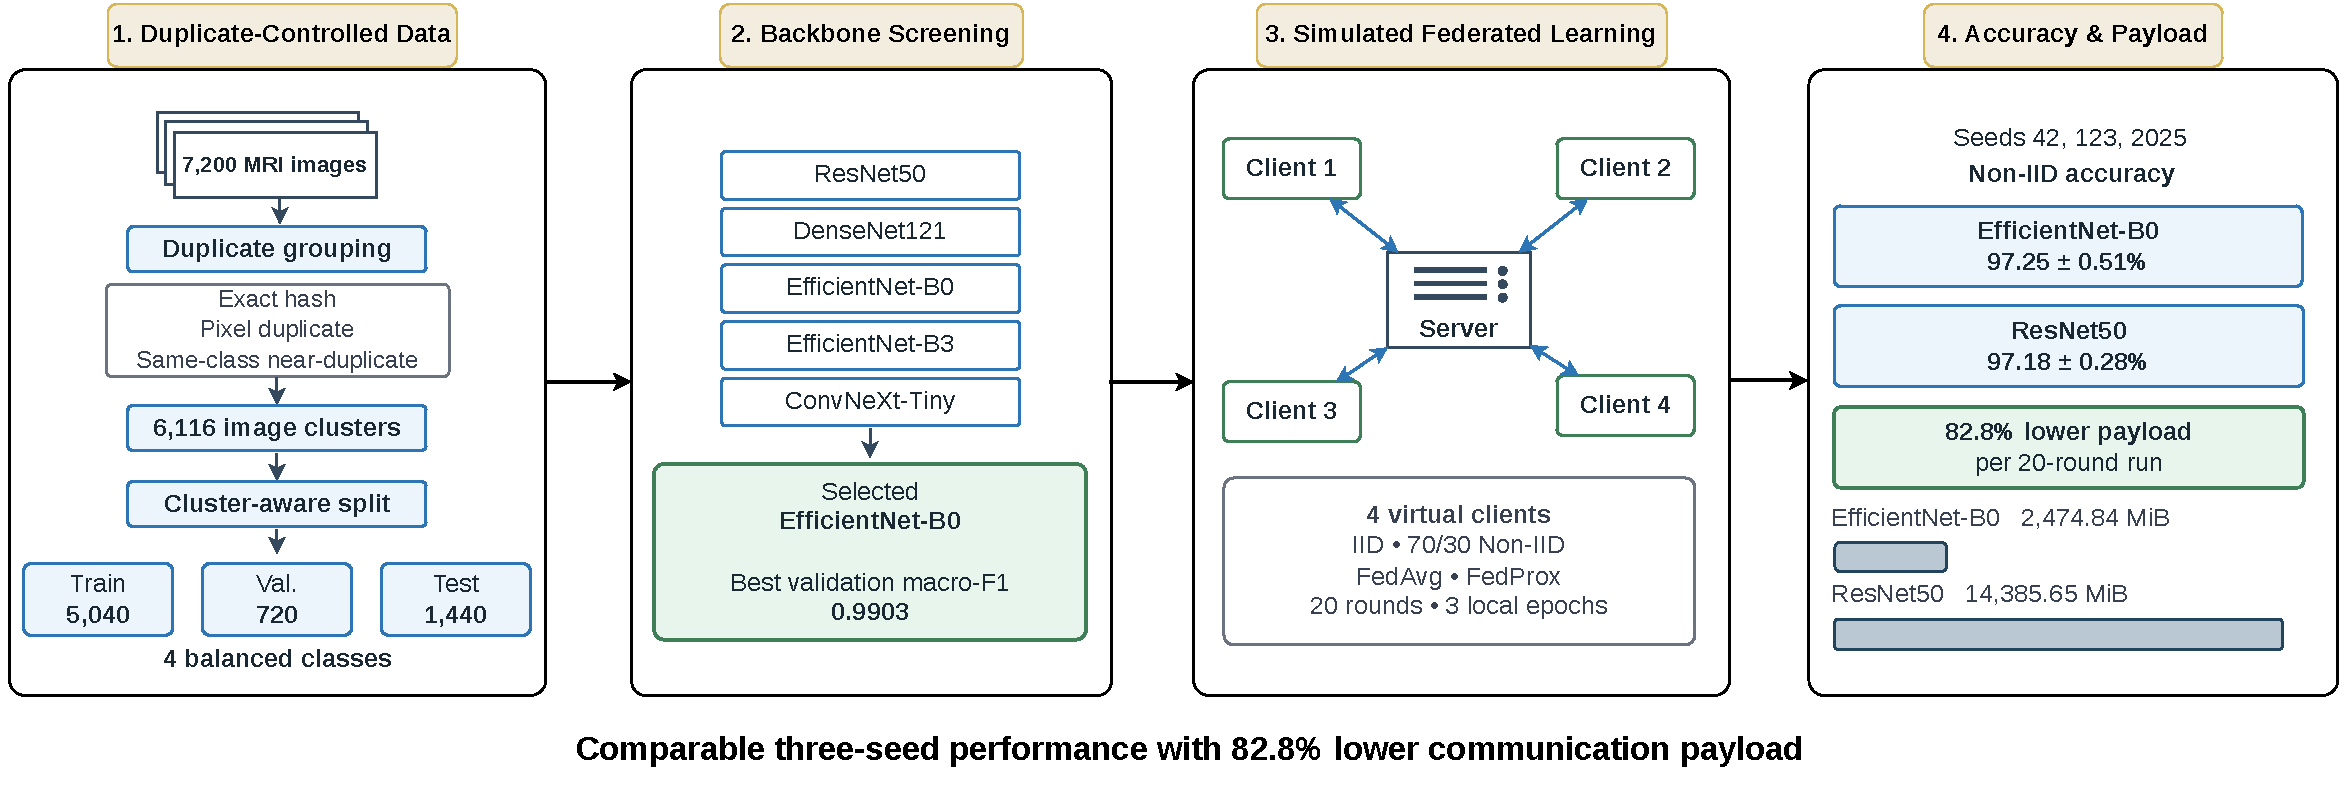
\includegraphics[width=\textwidth]{figures/federated_mri_pipeline.pdf}
\caption{Overview of the experimental workflow: duplicate-controlled split construction, centralized backbone screening, simulated federated learning with four virtual clients, and three-seed accuracy--communication comparison.}
\label{fig:pipeline}
\end{figure*}

\subsection{Dataset and Cluster-Aware Duplicate-Controlled Split}
We used the balanced Version~2 Kaggle snapshot, verified on June 28, 2026, containing 7,200 images (1,800 per class) \cite{nickparvar_brain_tumor_mri}. This version and count differ from the older 7,023-image release described in parts of the literature \cite{mastoi2025explainable}. The analysis used only the released images and class labels; no separate patient identifiers or linked clinical records were used.

We built the split around duplicate groups rather than individual files. All 7,200 images were represented as vertices in a graph. An edge joined a pair when it was an exact SHA-256 duplicate, pixel-identical after RGB resizing to $224\times224$, or a conservative same-class near duplicate satisfying both dHash distance $\leq5$ and grayscale SSIM $\geq0.92$ at $224\times224$. The thresholds were selected conservatively, and candidate near-duplicate edges were restricted to same-class image pairs satisfying both conditions. The resulting connected components formed 6,116 clusters; 596 contained multiple images, and the largest contained 14. Each cluster was assigned intact to one split, following the leakage-control motivation of duplicate-removal and patient-wise partitioning work \cite{melo2026exploiting,siam2026brain}.

Cluster assignment used 200 deterministic trials. Within trial $q$, seed $42+1009q$ provided random tie-breaking after clusters were ordered by decreasing size. Each cluster was greedily placed in the split that minimized normalized squared deviations from the class-wise and total-size targets, with additional penalties for overshoot. The assignment with the lowest objective was retained, using maximum class and total deviations as secondary criteria; the selected trial reached the exact class counts in Table~\ref{tab:split-counts} without dividing a cluster.

Cluster assignment preserved class balance while keeping every detected duplicate family within one partition. The final split contains 5,040 training, 720 validation, and 1,440 test images: 1,260, 180, and 360 images per class, respectively. Post-split checks found no exact, resized-pixel, or threshold-defined near-duplicate overlap across splits. This controls the forms of leakage that were measured; without patient identifiers, it cannot prove patient-level independence or substitute for an external cohort.

Table~\ref{tab:split-counts} reports the resulting class-balanced train, validation, and test partitions.

\begin{table}[t]
\centering
\caption{Class distribution in the cluster-aware duplicate-controlled split.}
\label{tab:split-counts}
\scriptsize
\setlength{\tabcolsep}{2pt}
\begin{tabular*}{\columnwidth}{@{\extracolsep{\fill}}|l|r|r|r|r|r|}
\hline
Split & Glioma & Meningioma & No tumor & Pituitary & Total \\
\hline
Train & 1,260 & 1,260 & 1,260 & 1,260 & 5,040 \\
\hline
Validation & 180 & 180 & 180 & 180 & 720 \\
\hline
Test & 360 & 360 & 360 & 360 & 1,440 \\
\hline
\end{tabular*}
\end{table}

\subsection{Centralized Backbone Screening}
Centralized screening selected the compact candidate before the final federated comparison. Five ImageNet-pretrained backbones were trained with $224\times224$ inputs, AdamW, and early stopping on validation macro-F1. ResNet50 served as the heavier residual baseline \cite{he2016resnet}, while EfficientNet-B0 served as the compact compound-scaled candidate \cite{tan2019efficientnet,abubakr2026explainable}. The test set was not used to rank candidate configurations; only the selected centralized model received a final test evaluation.

Centralized and federated training used the same ordered transformations: resize to $256\times256$; random resized crop to $224\times224$ with scale $(0.85,1.0)$; random horizontal flip ($p=0.5$); random rotation within $\pm15^\circ$; color jitter with brightness and contrast 0.2; tensor conversion; and ImageNet normalization with mean $(0.485,0.456,0.406)$ and standard deviation $(0.229,0.224,0.225)$. Validation and test used resize to $256\times256$, center crop to $224\times224$, tensor conversion, and the same normalization. Unlisted transformation arguments used torchvision defaults.

Table~\ref{tab:screening} reports the best predefined validation configuration for each backbone. EfficientNet-B0 at learning rate 0.0003 recorded the highest validation macro-F1, 0.990262, and was selected before FL evaluation. Its centralized test accuracy and macro-F1 were both 97.71\%. The ResNet50 row is the better of the tested layer4+fc and layer3+layer4+fc scopes; all other backbones were fully fine-tuned. Screening used one seed and served only as preliminary candidate selection, so its small validation differences do not establish a statistical ranking among backbones.

\begin{table}[!t]
\centering
\caption{Centralized backbone screening on the duplicate-controlled split. The best predefined validation configuration for each backbone is reported.}
\label{tab:screening}
\scriptsize
\setlength{\tabcolsep}{1.5pt}
\begin{tabularx}{\columnwidth}{|Y|L{1.24cm}|C{0.80cm}|C{0.82cm}|C{0.96cm}|}
\hline
Backbone & Scope & LR & \shortstack{Params.\\(M)} & \shortstack{Val.\\macro-F1} \\
\hline
ResNet50 & \shortstack[l]{layer3--4\\+ fc} & 0.0001 & 23.516 & 0.975004 \\
\hline
DenseNet121 & all & 0.0003 & 6.958 & 0.977831 \\
\hline
EfficientNet-B0 & all & 0.0003 & 4.013 & 0.990262 \\
\hline
EfficientNet-B3 & all & 0.0001 & 10.702 & 0.984731 \\
\hline
ConvNeXt-Tiny & all & 0.0001 & 27.823 & 0.988885 \\
\hline
\end{tabularx}
\end{table}

\subsection{Simulated Federated Learning Setup}
The federated protocol changes the backbone while holding optimization and participation fixed. All four virtual clients participate in each of 20 communication rounds. Every round uses three local epochs, batch size 32, AdamW, learning rate 0.0003, and weight decay 0.0001. The shared optimizer settings were deliberate: no backbone-specific FL tuning was performed, so optimization remained matched while the backbone changed. Centralized optima were not transferred because screening used different fine-tuning scopes and optimization conditions. Runs begin independently from ImageNet-pretrained weights, not from the centralized brain-MRI checkpoint.

Saved partitions keep client assignment from becoming a backbone-specific source of variation. The IID partition distributes each class approximately evenly. The Non-IID partition imposes 70/30 label skew: each client has one dominant class with 882 images and receives 126 images from each of the other three classes, for 1,260 images in total. At seeds 42, 123, and 2025, both backbones load the same saved Non-IID partition for that seed. Seed-42 IID FedAvg and Non-IID FedProx runs with EfficientNet-B0 provide supporting context. The clients represent controlled label imbalance, not differences among real institutions.

For FedAvg, the server aggregated full model state dictionaries using sample-count-weighted averaging \cite{mcmahan2017fedavg}:
\begin{equation}
    w^{(t+1)} = \sum_{k=1}^{K} \frac{n_k}{\sum_j n_j} w_k^{(t+1)},
\end{equation}
where $K$ is the number of clients, $n_k$ is the number of samples on client $k$, and $w_k^{(t+1)}$ is the locally updated model state. FedProx used the same aggregation rule with proximal coefficient $\mu=0.01$ during local optimization \cite{li2020fedprox}. It is included as a heterogeneous-FL baseline, not because it improved the final result in this experiment.

Model selection and test evaluation were kept separate. Validation macro-F1 selected the best global round, after which the fixed test set was evaluated once. Three-seed summaries use the mean and sample standard deviation with denominator $n-1$. Stable sample identifiers align predictions from the two backbones. For each seed, we use an exact two-sided McNemar test and 10,000 class-stratified paired-bootstrap resamples; both models receive the same sampled image indices. Holm adjustment covers the three seed-specific McNemar tests, and 95\% percentile intervals describe EfficientNet-B0-minus-ResNet50 differences in accuracy and macro-F1.

The seed-123 and seed-2025 runs used an NVIDIA GeForce RTX 5070 Ti with Python 3.14.6, PyTorch 2.12.1, torchvision 0.27.1, CUDA 13.0, and cuDNN 9.2. Their four training runs required 710--737 seconds each. The original seed-42 training environment was not retained, so its runtime is not compared with the new runs. Full configurations, split manifests, saved client assignments, per-image predictions, and analysis scripts are retained as reproducibility artifacts. Perfect bit-for-bit agreement is not guaranteed across different hardware, drivers, CUDA, cuDNN, or framework versions.

\subsection{Communication Accounting}
Communication accounting measures the tensor payload produced by the selected backbone. For state size $S$, $K$ clients, and $R$ rounds, one complete download and upload per client gives $2SKR$ bytes per run. We obtain $S$ by summing tensor bytes in the model's full \texttt{state\_dict}. With four clients and 20 rounds, each reported value includes every server-to-client download and client-to-server upload. It excludes headers, serialization, latency, compression, packet loss, and secure aggregation; the quantity is therefore full-state tensor payload rather than complete network performance \cite{radhika2026communication,zhou2022communication,das2026federated}.

\section{Results and Discussion}
\subsection{Centralized Model Selection}
The centralized benchmark was used to choose a compact candidate, not to make the final federated claim. Table~\ref{tab:screening} shows that EfficientNet-B0 had the highest validation macro-F1, 0.990262, among the predefined configurations. The selected model then achieved 97.71\% test accuracy and macro-F1. This result justifies carrying EfficientNet-B0 into the federated comparison; it does not make the backbone universally preferable.

\subsection{20-Round Federated Results}
Table~\ref{tab:fl-results} separates the matched three-seed comparison from two supporting seed-42 runs. The Non-IID FedAvg rows for EfficientNet-B0 and ResNet50 report means and sample standard deviations across seeds 42, 123, and 2025. IID FedAvg and Non-IID FedProx provide context only; they do not carry the evidential weight of the repeated comparison. Direct ranking against prior studies would also be misleading because their datasets, class definitions, client counts, and heterogeneity protocols differ.

\begin{table}[!t]
\centering
\caption{Final 20-round federated test results. Repeated rows report mean $\pm$ sample SD.}
\label{tab:fl-results}
\scriptsize
\setlength{\tabcolsep}{1.35pt}
\begin{tabularx}{\columnwidth}{|Y|C{0.55cm}|C{1.34cm}|C{1.34cm}|C{0.68cm}|C{1.28cm}|}
\hline
Experiment & Seeds & \shortstack{Acc.\\(\%)} & \shortstack{Macro-F1\\(\%)} & \shortstack{State\\(MiB)} & \shortstack{Payload\\(MiB/run)} \\
\hline
\shortstack[l]{FedAvg, Non-IID\\EfficientNet-B0} & 3 & $97.25\pm0.51$ & $97.25\pm0.51$ & 15.47 & 2,474.84 \\
\hline
\shortstack[l]{FedAvg, Non-IID\\ResNet50} & 3 & $97.18\pm0.28$ & $97.18\pm0.28$ & 89.91 & 14,385.65 \\
\hline
\shortstack[l]{FedAvg, IID\\EfficientNet-B0} & \shortstack{1\\(42)} & 97.92 & 97.92 & 15.47 & 2,474.84 \\
\hline
\shortstack[l]{FedProx, Non-IID\\EfficientNet-B0} & \shortstack{1\\(42)} & 97.64 & 97.64 & 15.47 & 2,474.84 \\
\hline
\end{tabularx}
\parbox{\columnwidth}{\scriptsize\textit{Note:} The repeated comparison uses seeds 42, 123, and 2025. IID and FedProx rows are single-seed supporting experiments. Communication payload is reported per 20-round federated run.}
\end{table}

Figure~\ref{fig:convergence} traces mean validation macro-F1 over the 20 communication rounds. The shaded bands show seed-to-seed variability on this fixed duplicate-controlled split; they should not be read as a general convergence guarantee.

\begin{figure}[!t]
\centering
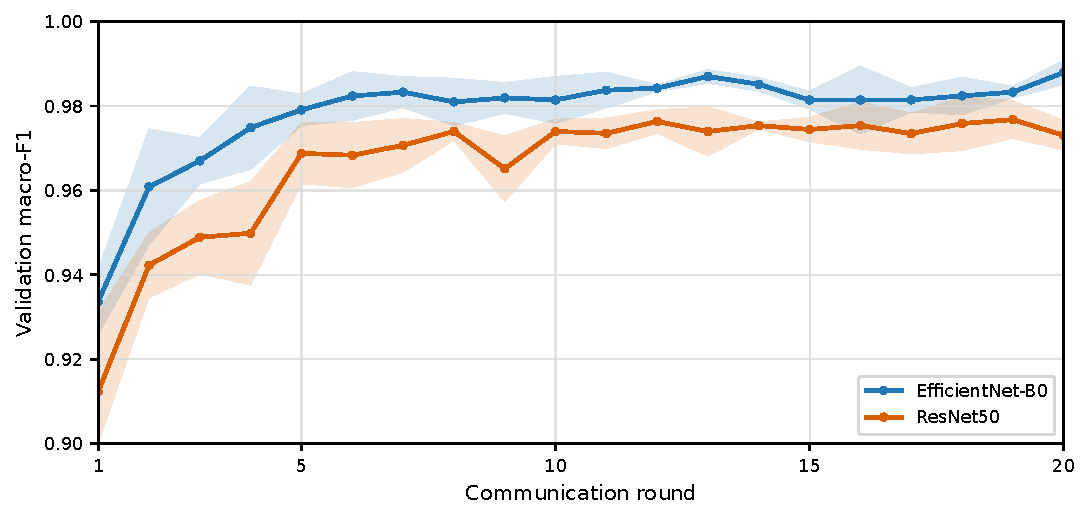
\includegraphics[width=\columnwidth]{figures/fig_multiseed_convergence.pdf}
\caption{Mean validation macro-F1 across three seeds under the Non-IID FedAvg setting; shaded regions denote $\pm1$ sample standard deviation. The vertical axis is restricted to 0.90--1.00 for readability.}
\label{fig:convergence}
\end{figure}

Across the three seeds, the two backbones produced nearly the same aggregate classification result. EfficientNet-B0 achieved $97.25\pm0.51$\% accuracy and macro-F1; ResNet50 achieved $97.18\pm0.28$\% for both metrics. The mean paired difference, EfficientNet-B0 minus ResNet50, was 0.07 percentage points for accuracy and macro-F1, with a 0.32-point sample SD for each. The direction changed with the seed: seed 42 favored EfficientNet-B0, seed 123 favored ResNet50, and seed 2025 tied in accuracy.

The paired analyses do not support an accuracy-superiority claim. At seeds 42, 123, and 2025, the accuracy differences were 0.42 points (95\% CI: $-0.42$ to 1.25), $-0.21$ points ($-1.11$ to 0.69), and 0.00 points ($-0.69$ to 0.69). The corresponding raw exact McNemar $p$-values were 0.405, 0.761, and 1.000; all Holm-adjusted values were 1.000. Macro-F1 differences were 0.41 points (95\% CI: $-0.40$ to 1.23), $-0.21$ points ($-1.11$ to 0.69), and approximately 0.00 points ($-0.69$ to 0.68). Every bootstrap interval included zero. No statistically distinguishable difference was detected for any seed, although this is not evidence of formal equivalence.

\subsection{Communication Comparison}
With client participation and round count fixed, payload follows directly from model state size. Figure~\ref{fig:comm} shows 2,474.84~MiB per 20-round run for EfficientNet-B0 and 14,385.65~MiB for ResNet50, a reduction of approximately 82.8\%. These are per-run values, not totals across the three seeds.

\begin{figure}[!t]
\centering
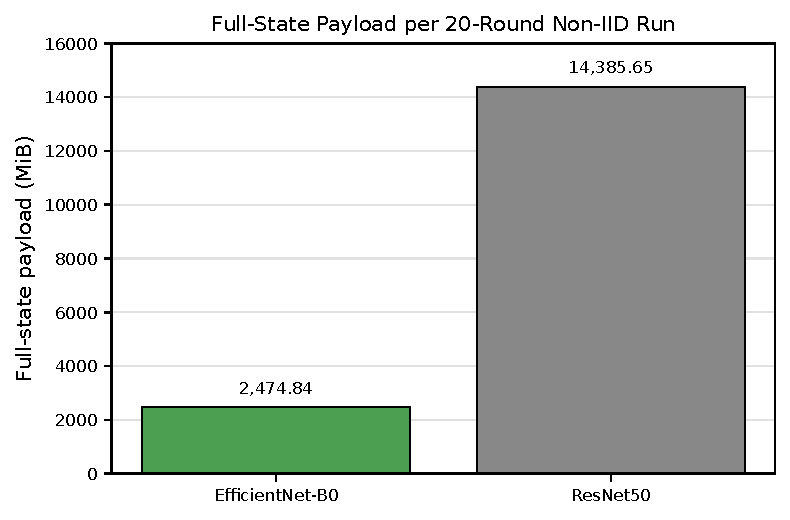
\includegraphics[width=0.95\columnwidth]{figures/fig_main_communication_comparison.pdf}
\caption{Total full-state communication payload per 20-round Non-IID FedAvg run.}
\label{fig:comm}
\end{figure}

The gap comes from the backbones' different footprints. EfficientNet-B0 has 4.01M parameters and a 15.47~MiB state; ResNet50 has 23.52M parameters and an 89.91~MiB state. Complete upload and download in every round turn that state-size difference into a large tensor-payload difference, while observed classification performance remains comparable. The result says nothing about end-to-end latency and does not show statistically superior accuracy.

\subsection{Class-Wise Behavior}
Figure~\ref{fig:cm} provides a seed-42 class-wise diagnostic for the selected Non-IID FedAvg EfficientNet-B0 model. Diagonal counts remain high across all four classes, with 348/360 correct glioma predictions, 346/360 meningioma, 354/360 no-tumor, and 358/360 pituitary. The largest off-diagonal counts are eight glioma images predicted as meningioma and nine meningioma images predicted as pituitary, while no-tumor and pituitary errors remain sparse. This pattern is consistent with the strong aggregate macro-F1, but it is descriptive only: one seed-level confusion matrix does not replace the repeated paired comparison or constitute clinical validation.

\begin{figure}[!ht]
\centering
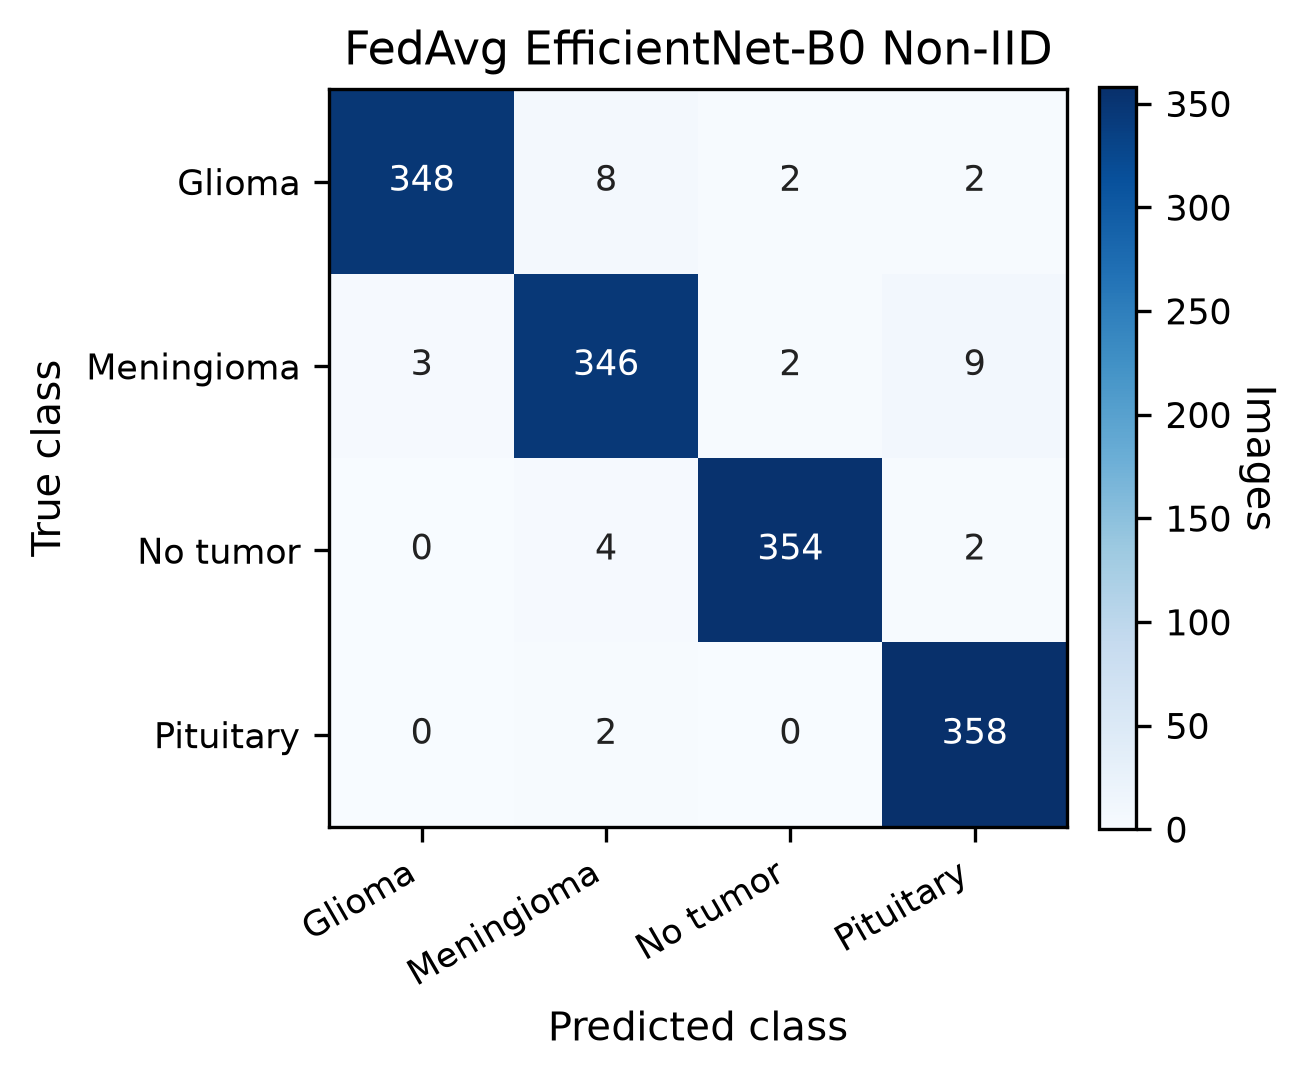
\includegraphics[width=0.93\columnwidth]{figures/fig_confusion_matrix_efficientnet_b0_noniid.png}
\caption{Test confusion matrix for FedAvg EfficientNet-B0 under the 20-round Non-IID setting.}
\label{fig:cm}
\end{figure}

\section{Limitations}
Three seeds capture only a small part of the possible stochastic variation. The fixed 1,440-image test set also comes from one duplicate-controlled split of one public dataset family. Centralized screening used one seed, and the shared federated optimizer was not tuned separately for each backbone; conclusions therefore apply to the predefined matched schedule rather than each model's individually optimized setting. Because we performed neither an equivalence nor a non-inferiority test, ``not statistically distinguishable'' must not be read as proof of equivalence.

The simulation cannot establish institutional or clinical generalization. Four label-skewed virtual clients do not reproduce cross-hospital differences in scanners, acquisition protocols, populations, or governance \cite{naseer2026medfl,xu2023federated}. Duplicate control removes the cross-split overlaps detected by our rules, but it cannot eliminate every dataset bias or establish patient independence without metadata. No external cohort, prospective evaluation, or radiologist comparison was available.

The communication analysis measures tensor payload rather than complete networking performance. It excludes latency, bandwidth variation, serialization overhead, energy, packet loss, client availability, secure aggregation, and differential-privacy overhead \cite{rieke2020future,radhika2026communication,aniket2025cfl}. Standard FL can also leak information through transmitted updates. Our results therefore establish neither complete privacy protection nor legal compliance.

\FloatBarrier
\section{Conclusion}
This study isolated the effect of backbone choice on full-state payload under a duplicate-controlled, matched FL evaluation. Across three seeds, EfficientNet-B0 and ResNet50 achieved comparable Non-IID accuracy and macro-F1, while EfficientNet-B0 reduced measured full-state tensor payload per 20-round run by approximately 82.8\%. Beyond this model pair, the protocol provides a reproducible template for combining duplicate control, matched partitions, repeated runs, and paired statistical analysis in federated medical-imaging comparisons. The result supports communication-aware compact-backbone selection in this simulation; evaluation on independent institutional cohorts, additional seeds, and broader heterogeneity settings remains necessary.

\bibliographystyle{IEEEtran}
\bibliography{references}

\end{document}
